\documentclass[12pt,a4paper]{article}
\usepackage[utf8]{inputenc}
\usepackage[english]{babel}
\usepackage{amsmath}
\usepackage{amsfonts}
\usepackage{amssymb}
\usepackage{graphicx}
\usepackage{listings}
\usepackage{xcolor}
\usepackage{geometry}
\usepackage{fancyhdr}
\usepackage[hidelinks]{hyperref}
\usepackage{booktabs}
\usepackage{array}
\usepackage{longtable}

% Page geometry
\geometry{margin=2.5cm}

% Header and footer
\pagestyle{fancy}
\fancyhf{}
\rhead{Nicolas Leone - 1986354}
\lhead{Cybersecurity HW02}
\cfoot{\thepage}

% Code listing style
\lstdefinestyle{cstyle}{
    language=C,
    basicstyle=\ttfamily\footnotesize,
    keywordstyle=\color{blue}\bfseries,
    commentstyle=\color{gray}\itshape,
    stringstyle=\color{red},
    numbers=left,
    numberstyle=\tiny\color{gray},
    stepnumber=1,
    numbersep=5pt,
    backgroundcolor=\color{lightgray!10},
    frame=single,
    frameround=tttt,
    breaklines=true,
    breakatwhitespace=false,
    showstringspaces=false,
    tabsize=4,
    captionpos=b
}

\lstset{style=cstyle}

\title{Homework 02: Comparing Symmetric Cipher Algorithms Performance}
\author{Nicolas Leone\\Student ID: 1986354\\Cybersecurity}
\date{\today}

\begin{document}

\maketitle

\tableofcontents
\newpage

\section{Introduction}

\subsection{Overview}
Symmetric encryption is a fundamental component of modern cryptography, where the same key is used for both encryption and decryption operations. This homework focuses on comparing the performance characteristics of three widely-used symmetric cipher algorithms: AES (Advanced Encryption Standard), SM4, and Camellia. All three algorithms operate in CBC (Cipher Block Chaining) mode with 128-bit keys.

The objective of this study is to measure and analyze the encryption and decryption performance of these algorithms across different file sizes, providing insights into their computational efficiency and practical applicability in real-world scenarios.

\subsection{AES-128-CBC (Advanced Encryption Standard)}
AES is one of the most widely adopted encryption standards worldwide, established by NIST in 2001. It replaced the older DES (Data Encryption Standard) and has become the de facto standard for symmetric encryption in both government and commercial applications.

\textbf{Key characteristics:}
\begin{itemize}
    \item \textbf{Block size:} 128 bits
    \item \textbf{Key size:} 128 bits (in this study)
    \item \textbf{Structure:} Substitution-Permutation Network (SPN)
    \item \textbf{Rounds:} 10 rounds for 128-bit keys
    \item \textbf{Security:} Proven security with no practical attacks on full AES
    \item \textbf{Hardware support:} Widely implemented in modern processors (AES-NI instructions)
\end{itemize}

AES operates through multiple rounds of substitution, permutation, mixing, and key addition operations. Its widespread adoption and hardware acceleration make it typically the fastest option among secure symmetric ciphers.

\subsection{SM4-128-CBC}
SM4 is a block cipher developed by the Chinese government in 2006 and was established as a Chinese national encryption standard (GB/T 32907-2016). It was designed as an alternative to AES for use in Chinese commercial and government applications.

\textbf{Key Characteristics:}
\begin{itemize}
    \item \textbf{Block Size}: 128 bits
    \item \textbf{Key Size}: 128 bits (fixed)
    \item \textbf{Structure}: 32 rounds of Feistel-like structure with substitution-permutation network (SPN)
    \item \textbf{Security Level}: Comparable to AES-128
    \item \textbf{Standardization}: Chinese national standard (GB/T 32907-2016), ISO/IEC 18033-3:2010
\end{itemize}

SM4 uses a structure with 32 rounds and employs S-boxes and linear transformations similar to AES. It was designed to be efficient in both software and hardware implementations, though it lacks the widespread hardware acceleration of AES.

\subsection{Camellia-128-CBC}
Camellia is a block cipher jointly developed by Mitsubishi Electric and NTT in Japan in 2000. It has been approved for use by ISO/IEC, the European NESSIE project, and the Japanese CRYPTREC project, demonstrating its international recognition.

\textbf{Key characteristics:}
\begin{itemize}
    \item \textbf{Block size:} 128 bits
    \item \textbf{Key size:} 128 bits (in this study)
    \item \textbf{Structure:} Feistel network
    \item \textbf{Rounds:} 18 rounds for 128-bit keys
    \item \textbf{Security:} Comparable to AES with similar security margins
    \item \textbf{Hardware support:} Some hardware implementations available
\end{itemize}

Camellia uses a Feistel structure (unlike AES's SPN structure and SM4's Feistel-like structure) and includes logical operations that provide good performance on various platforms. It is particularly popular in Japan and has been adopted in several security protocols.

\subsection{CBC Mode (Cipher Block Chaining)}
All three algorithms in this study operate in CBC mode, which is one of the most common block cipher modes of operation. In CBC mode:
\begin{itemize}
    \item Each plaintext block is XORed with the previous ciphertext block before encryption
    \item An Initialization Vector (IV) is used for the first block
    \item This creates a dependency chain, making identical plaintext blocks produce different ciphertext
\end{itemize}

\textbf{Security Considerations for CBC Mode:}
\begin{itemize}
    \item The IV must be unpredictable and unique for each encryption operation with the same key
    \item Using a random IV ensures that encrypting the same plaintext multiple times produces different ciphertext
    \item Our implementation generates a new random IV for each file and algorithm combination using OpenSSL's \texttt{RAND\_bytes()}
\end{itemize}

\newpage

\section{Implementation}

\subsection{Development Environment}
The performance comparison was implemented in C using the OpenSSL cryptographic library (version 3.6.0). The program was compiled using GCC with optimization flags and executed on macOS with an ARM64 architecture processor.

\subsection{Source Code}
The complete implementation consists of several key components: file I/O operations, encryption/decryption functions and performance measurement utilities. Below is the full source code with detailed explanations.

\lstinputlisting[language=C, caption=Complete implementation of cipher performance comparison]{HW02_Nicolas_Leone_1986354.c}

\subsection{Code Explanation}

\subsubsection{Error Handling}
The \texttt{handle\_crypto\_error()} function provides centralized error handling for OpenSSL operations. When a cryptographic operation fails, this function prints the error stack from OpenSSL and terminates the program, ensuring that errors are immediately visible during testing.

\subsubsection{File Operations}
Two utility functions handle file I/O:
\begin{itemize}
    \item \texttt{load\_file\_content()}: Reads an entire file into memory. It uses \texttt{stat()} to determine file size, allocates appropriate memory, and loads the content into a buffer. Returns the file size or -1 on error.
    \item \texttt{save\_to\_file()}: Writes a data buffer to a file. While not used in the current performance tests, this function is included for completeness and potential future use.
\end{itemize}

\subsubsection{Encryption Function}
The \texttt{perform\_encryption()} function implements generic encryption for any EVP cipher:
\begin{enumerate}
    \item Creates a new cipher context using \texttt{EVP\_CIPHER\_CTX\_new()}
    \item Initializes encryption with \texttt{EVP\_EncryptInit\_ex()}, specifying the cipher algorithm, key, and IV
    \item Processes the plaintext with \texttt{EVP\_EncryptUpdate()}, which handles data in chunks
    \item Finalizes encryption with \texttt{EVP\_EncryptFinal\_ex()}, which processes any remaining data and applies padding
    \item Frees the cipher context and returns the total encrypted data length
\end{enumerate}

\subsubsection{Decryption Function}
The \texttt{perform\_decryption()} function mirrors the encryption process:
\begin{enumerate}
    \item Creates a new cipher context
    \item Initializes decryption with \texttt{EVP\_DecryptInit\_ex()}
    \item Processes ciphertext with \texttt{EVP\_DecryptUpdate()}
    \item Finalizes decryption with \texttt{EVP\_DecryptFinal\_ex()}, which also verifies and removes padding
    \item Frees the context and returns the plaintext length
\end{enumerate}

\subsubsection{Key Generation and Management}
The implementation follows the security best practice of generating a cryptographically secure random key at initialization:

\begin{itemize}
    \item A 128-bit (16-byte) symmetric key is randomly generated using OpenSSL's \texttt{RAND\_bytes()} function in the \texttt{main()} function
    \item The same randomly generated key is used for all encryption and decryption operations across all three algorithms and all test files
\end{itemize}

This approach ensures:
\begin{itemize}
    \item \textbf{Security}: The key is unpredictable and cannot be guessed
    \item \textbf{Realism}: Reflects real-world usage where keys are randomly generated, not hardcoded
\end{itemize}

For each encryption/decryption operation, a new random Initialization Vector (IV) is generated to ensure that encrypting the same plaintext multiple times produces different ciphertext, which is a fundamental requirement of CBC mode security.

\subsubsection{Main Processing Function}
The \texttt{process\_file\_with\_ciphers()} function orchestrates the entire testing process:
\begin{enumerate}
    \item Loads the input file into memory
    \item Allocates buffers for ciphertext and decrypted text (with extra space for padding)
    \item Defines the cipher array (AES, SM4, Camellia) and corresponding names
    \item For each algorithm:
    \begin{itemize}
        \item Generates a random 128-bit IV using \texttt{RAND\_bytes()}
        \item Measures encryption time using \texttt{clock\_gettime()} with \texttt{CLOCK\_MONOTONIC}
        \item Performs encryption
        \item Measures decryption time
        \item Performs decryption
        \item Verifies correctness by comparing decrypted text with original plaintext using \texttt{memcmp()}
    \end{itemize}
    \item Frees all allocated memory
\end{enumerate}

\subsubsection{Time Measurement}
High-precision time measurement is achieved using \texttt{clock\_gettime()} with the \texttt{CLOCK\_MONOTONIC} clock which captures time before and after each operation and calculates elapsed time in microseconds ($\mu$s).

\subsubsection{Test Files}
The program tests three files with different sizes:
\begin{itemize}
    \item \texttt{text\_16B.txt}: 16 bytes - represents small data encryption (e.g., passwords, tokens)
    \item \texttt{text\_20KB.txt}: 20 kilobytes - represents medium-sized data (e.g., configuration files, small documents)
    \item \texttt{binary\_2MB.bin}: 2 megabytes - represents large data encryption (e.g., images, compressed files)
\end{itemize}

The binary file was generated using random data from \texttt{/dev/urandom} to simulate realistic encrypted content with high entropy.

\newpage

\section{Results and Analysis}

The following charts present the encryption and decryption performance for each file size across all three algorithms. Time measurements are reported in microseconds ($\mu$s).

\subsection{Performance Analysis}

\subsubsection{Small File Performance (16 B)}
For the 16-byte file, all three algorithms demonstrate comparable performance:
\begin{itemize}
    \item \textbf{AES-128-CBC}: 3 $\mu$s encryption, 1 $\mu$s decryption
    \item \textbf{SM4-128-CBC}: 7 $\mu$s encryption, 2 $\mu$s decryption
    \item \textbf{Camellia-128-CBC}: 3 $\mu$s encryption, 1 $\mu$s decryption
\end{itemize}

\begin{figure}[h]
\centering
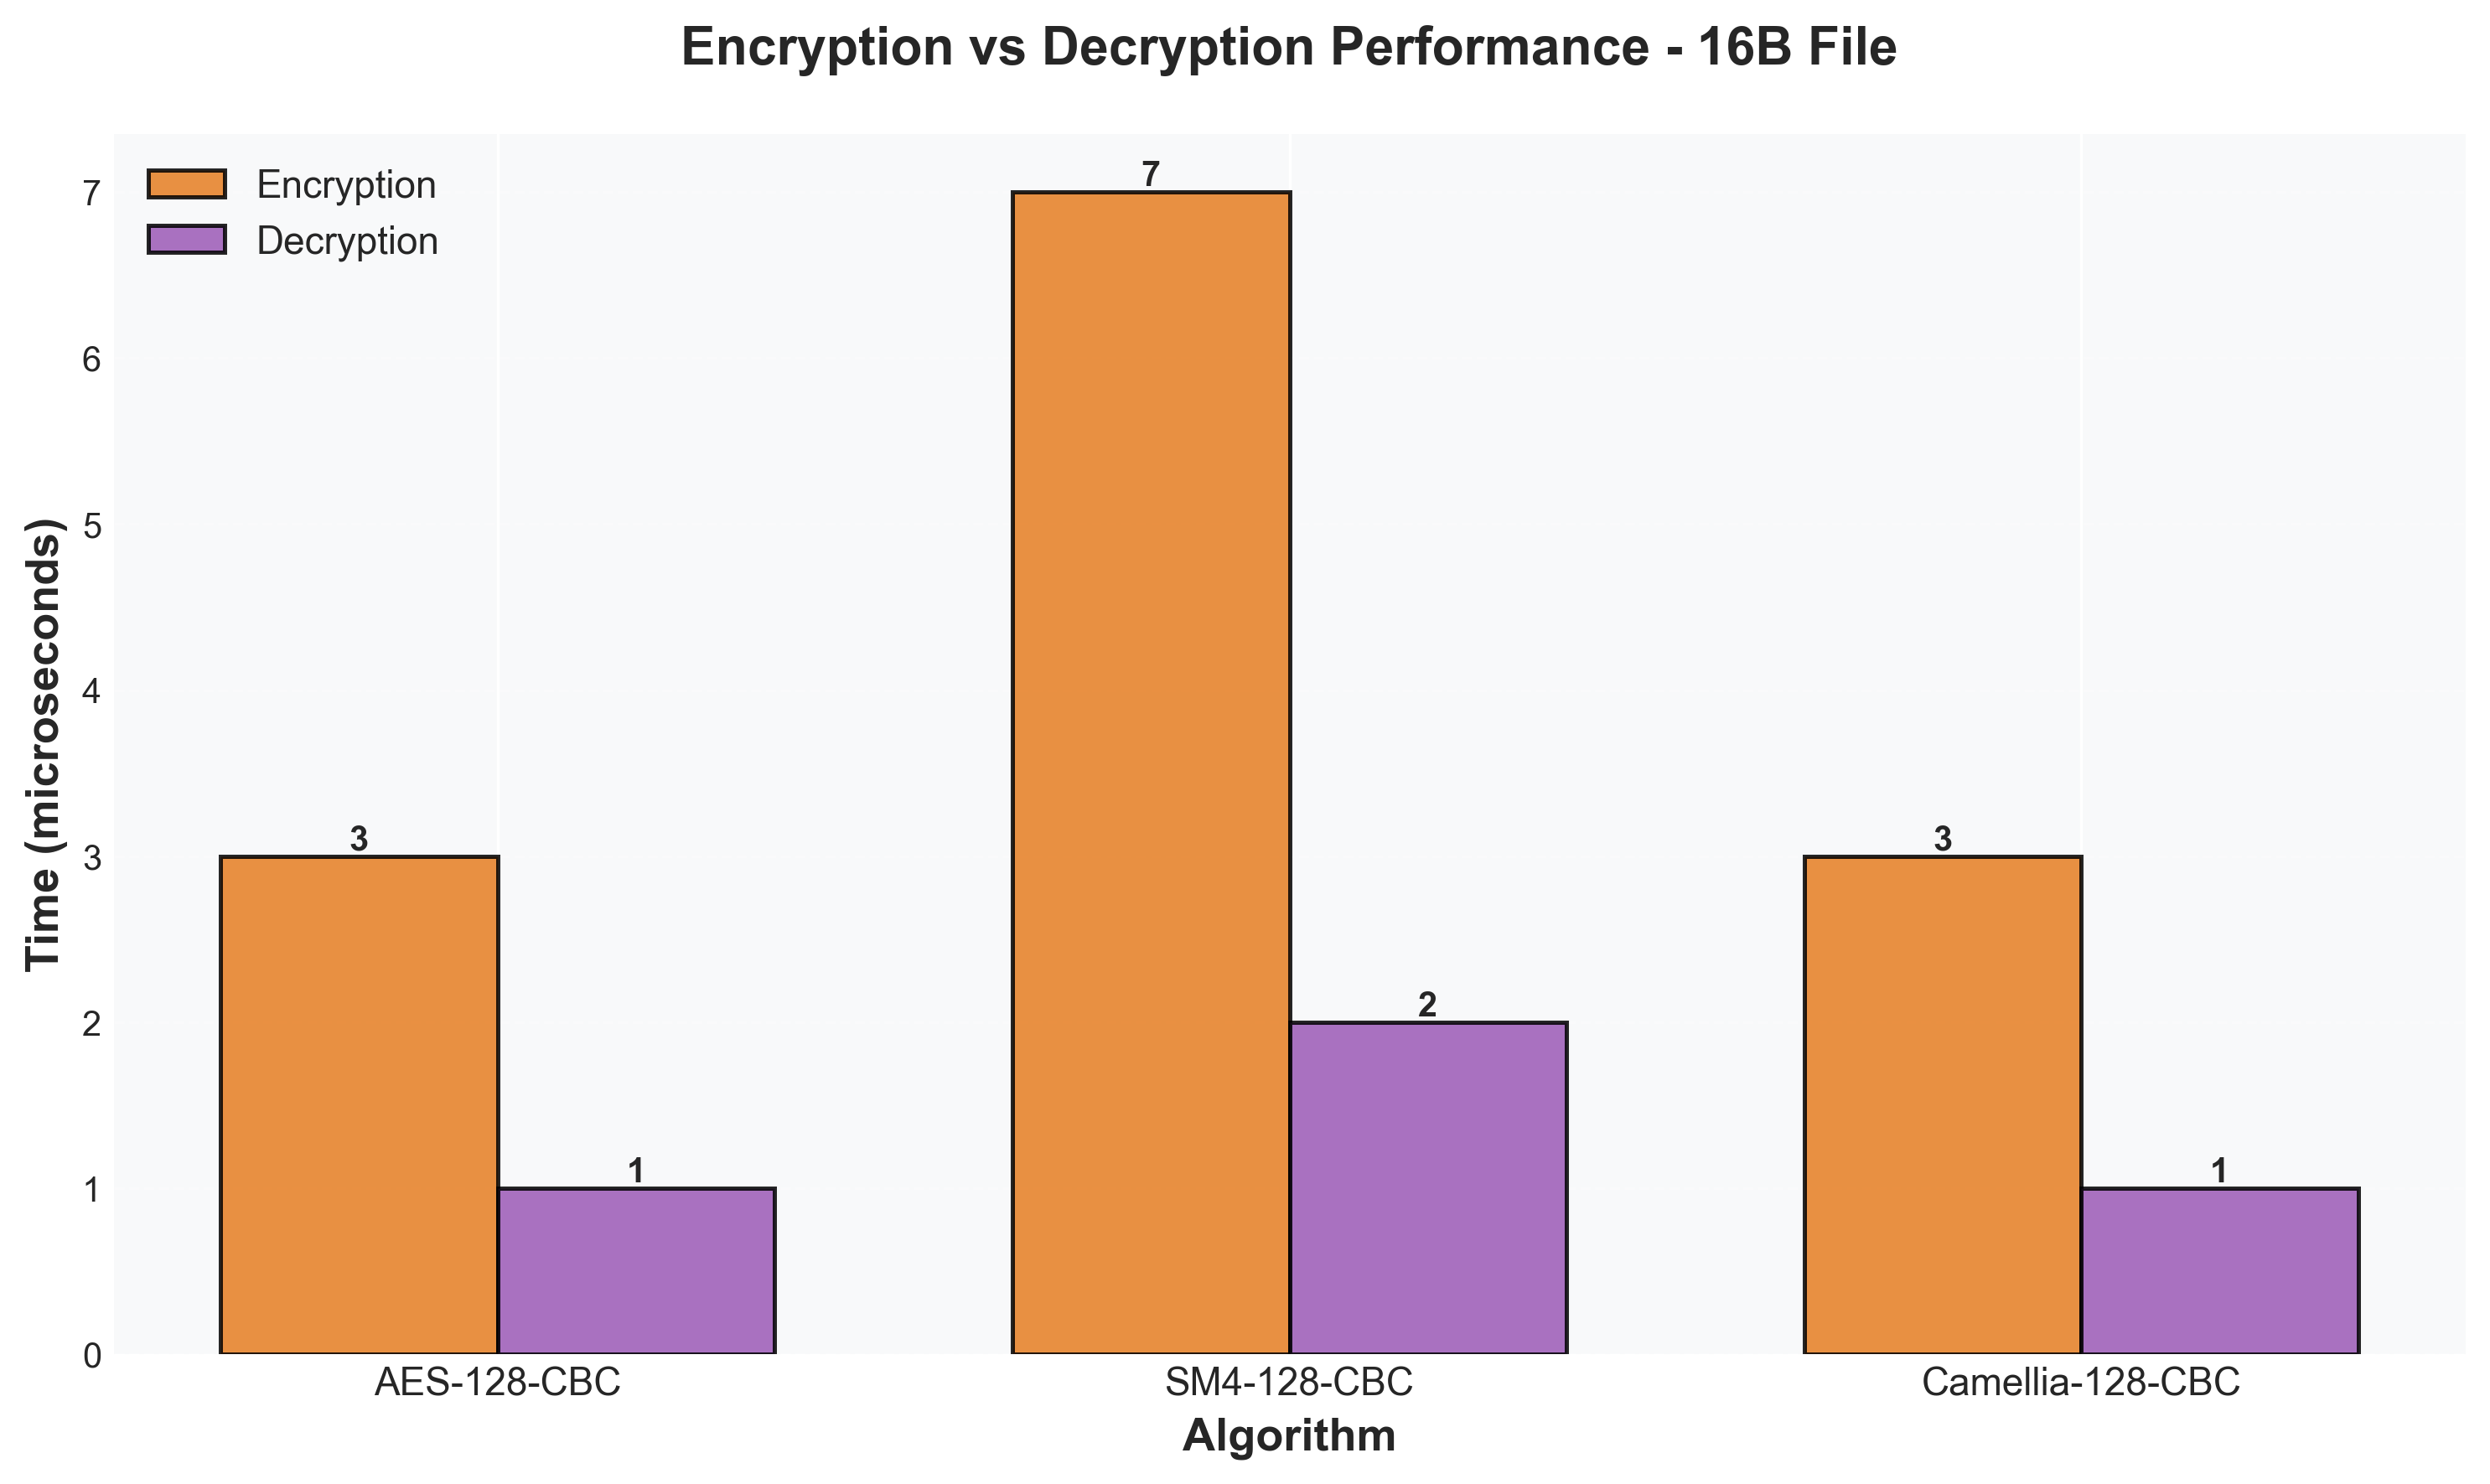
\includegraphics[width=0.85\textwidth]{performance_16B.png}
\caption{Encryption and Decryption performance for 16B file. At this small scale, all algorithms perform similarly with times in the single-digit microsecond range.}
\label{fig:perf_16b}
\end{figure}

At this scale, the overhead of context initialization and function calls dominates the actual cipher operations. AES and Camellia show identical performance, while SM4 exhibits slightly higher overhead. All algorithms complete operations in under 10 microseconds, making the differences negligible for practical purposes at this file size.

\subsubsection{Medium File Performance (20 KB)}
With a 20KB file, performance differences become more pronounced:
\begin{itemize}
    \item \textbf{AES-128-CBC}: 15 $\mu$s encryption, 5 $\mu$s decryption
    \item \textbf{SM4-128-CBC}: 166 $\mu$s encryption, 130 $\mu$s decryption
    \item \textbf{Camellia-128-CBC}: 120 $\mu$s encryption, 89 $\mu$s decryption
\end{itemize}

\begin{figure}[h]
\centering
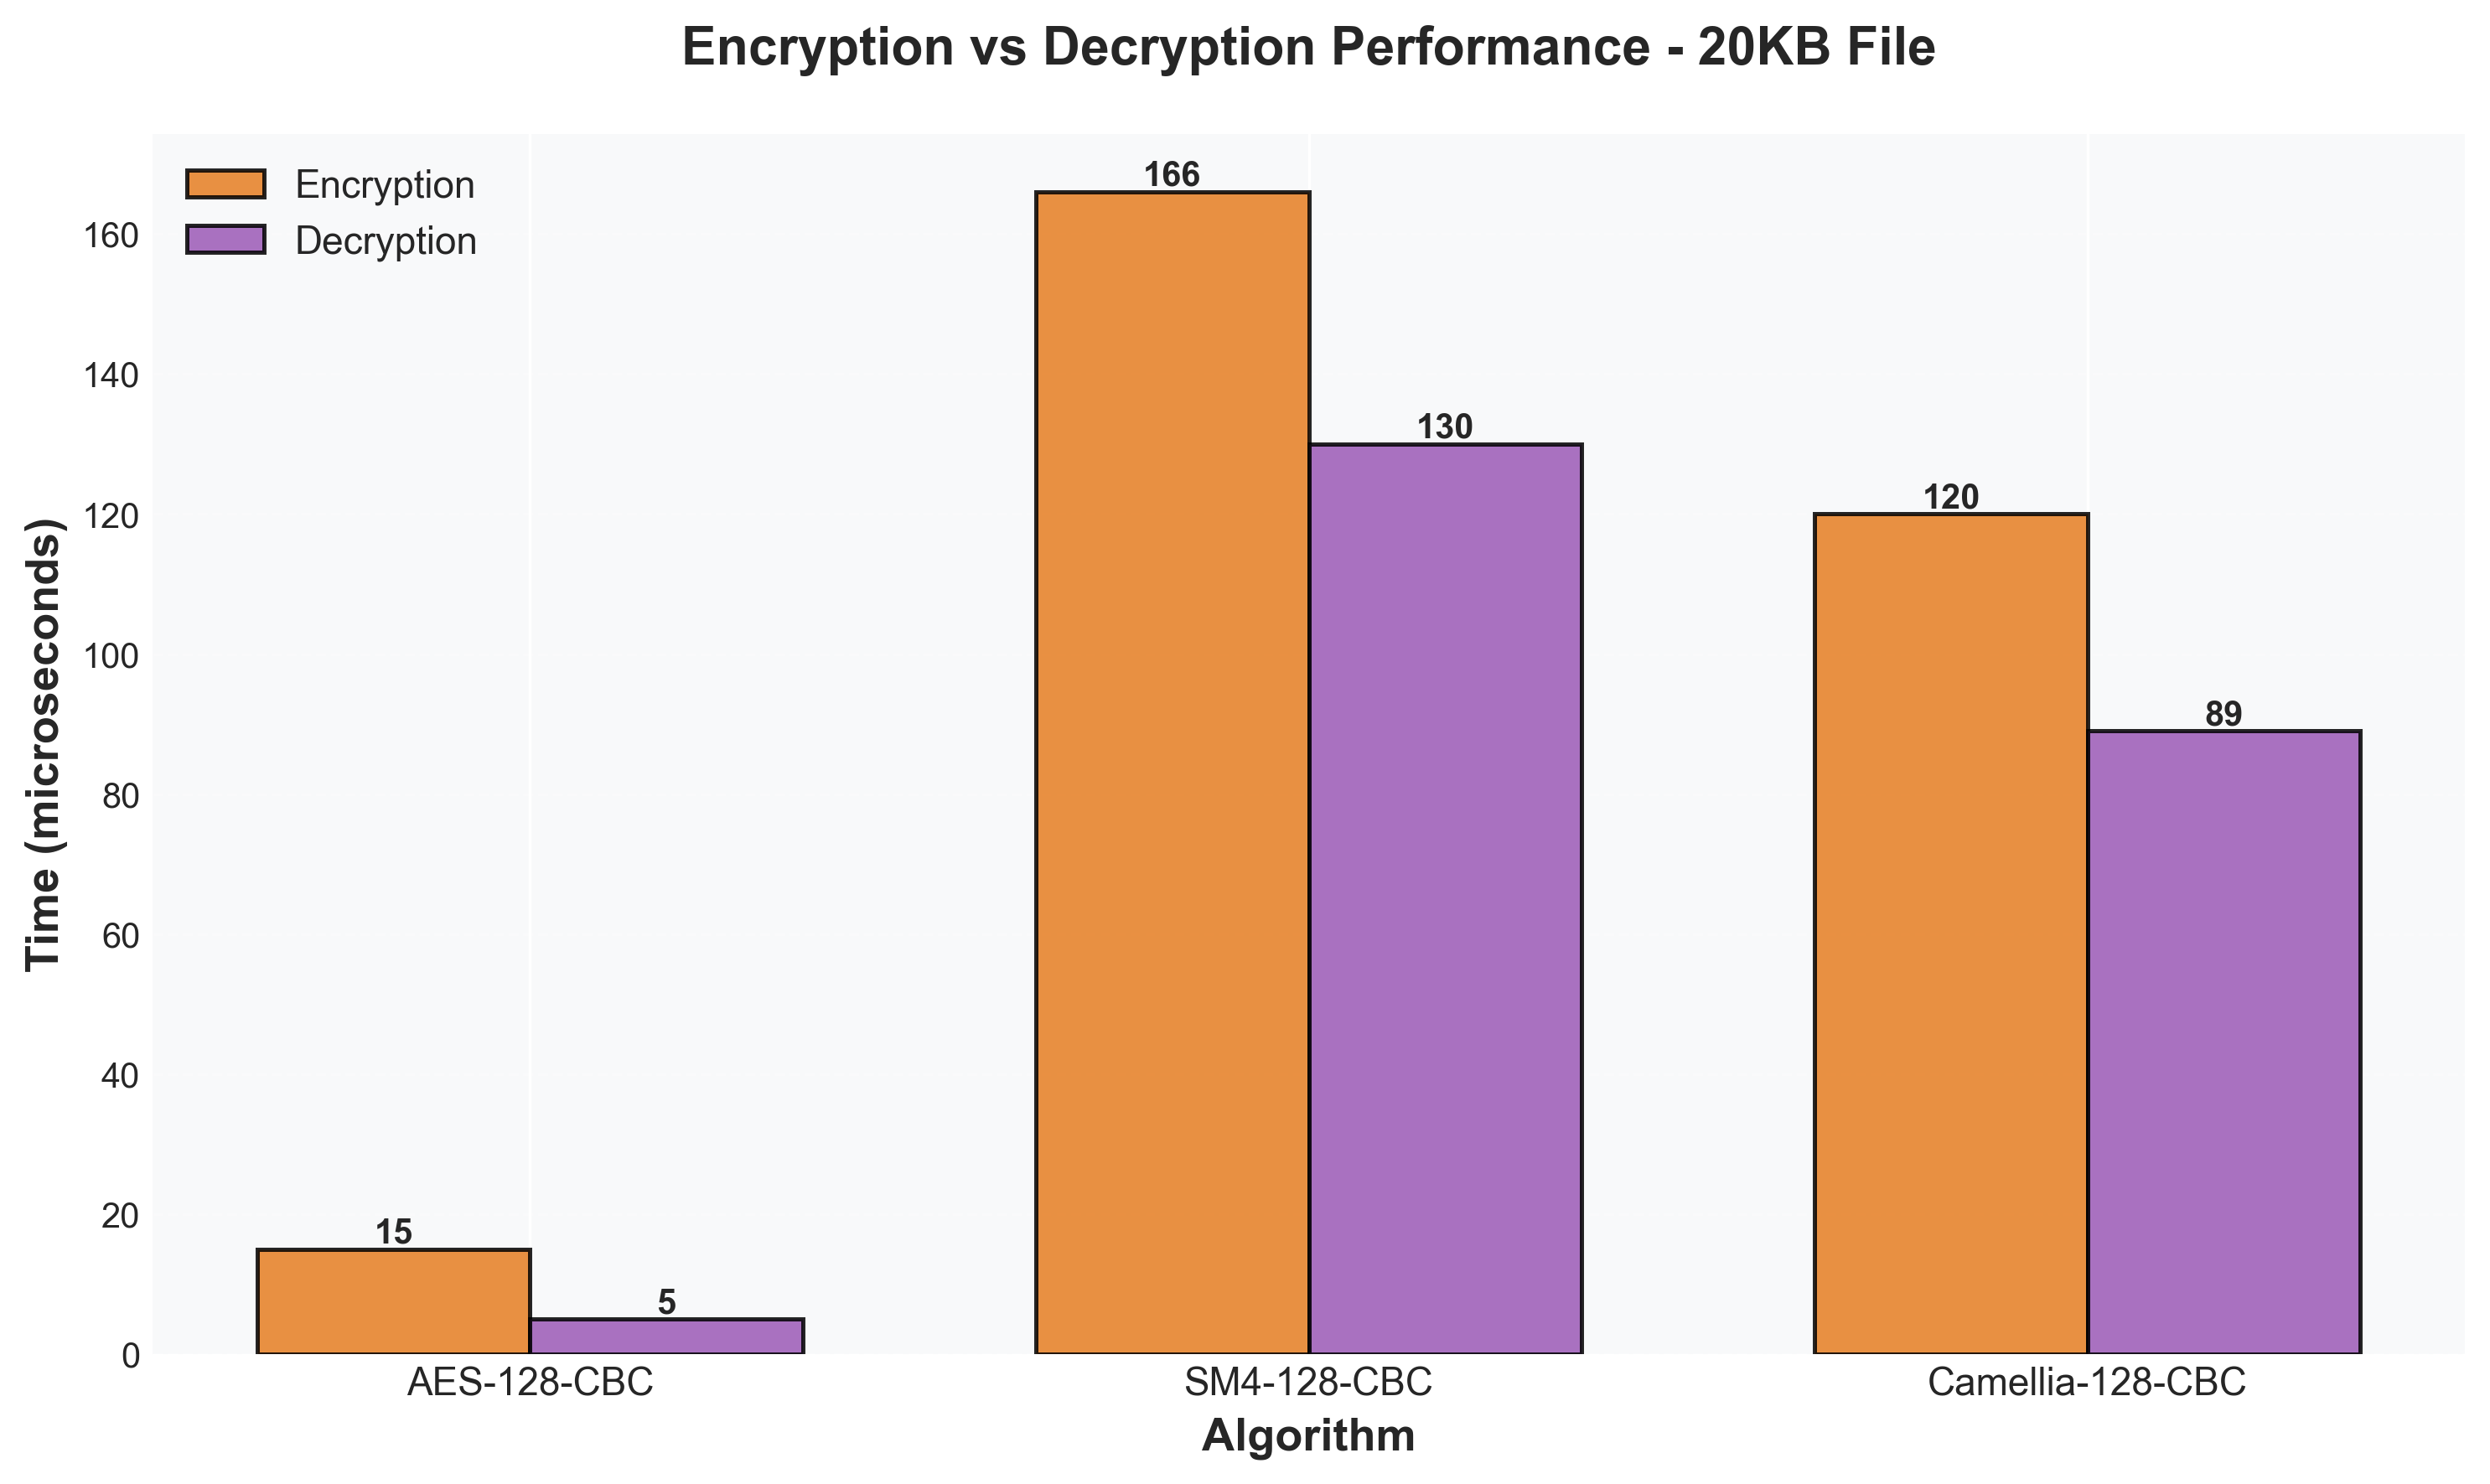
\includegraphics[width=0.85\textwidth]{performance_20KB.png}
\caption{Encryption and Decryption performance for 20KB file. Performance differences become more apparent, with AES showing clear advantages.}
\label{fig:perf_20kb}
\end{figure}

AES demonstrates approximately 8-11× faster performance than SM4 and Camellia. This advantage is likely due to hardware acceleration (AES-NI instructions) available on the test platform. Camellia performs approximately 1.4× better than SM4 at this scale, showing its efficiency advantage.

\subsubsection{Large File Performance (2 MB)}
The 2MB binary file reveals the most significant performance differences:
\begin{itemize}
    \item \textbf{AES-128-CBC}: 1,045 $\mu$s (1.05 ms) encryption, 241 $\mu$s (0.24 ms) decryption
    \item \textbf{SM4-128-CBC}: 15,788 $\mu$s (15.79 ms) encryption, 11,365 $\mu$s (11.37 ms) decryption
    \item \textbf{Camellia-128-CBC}: 8,843 $\mu$s (8.84 ms) encryption, 6,564 $\mu$s (6.56 ms) decryption
\end{itemize}

\begin{figure}[h]
\centering
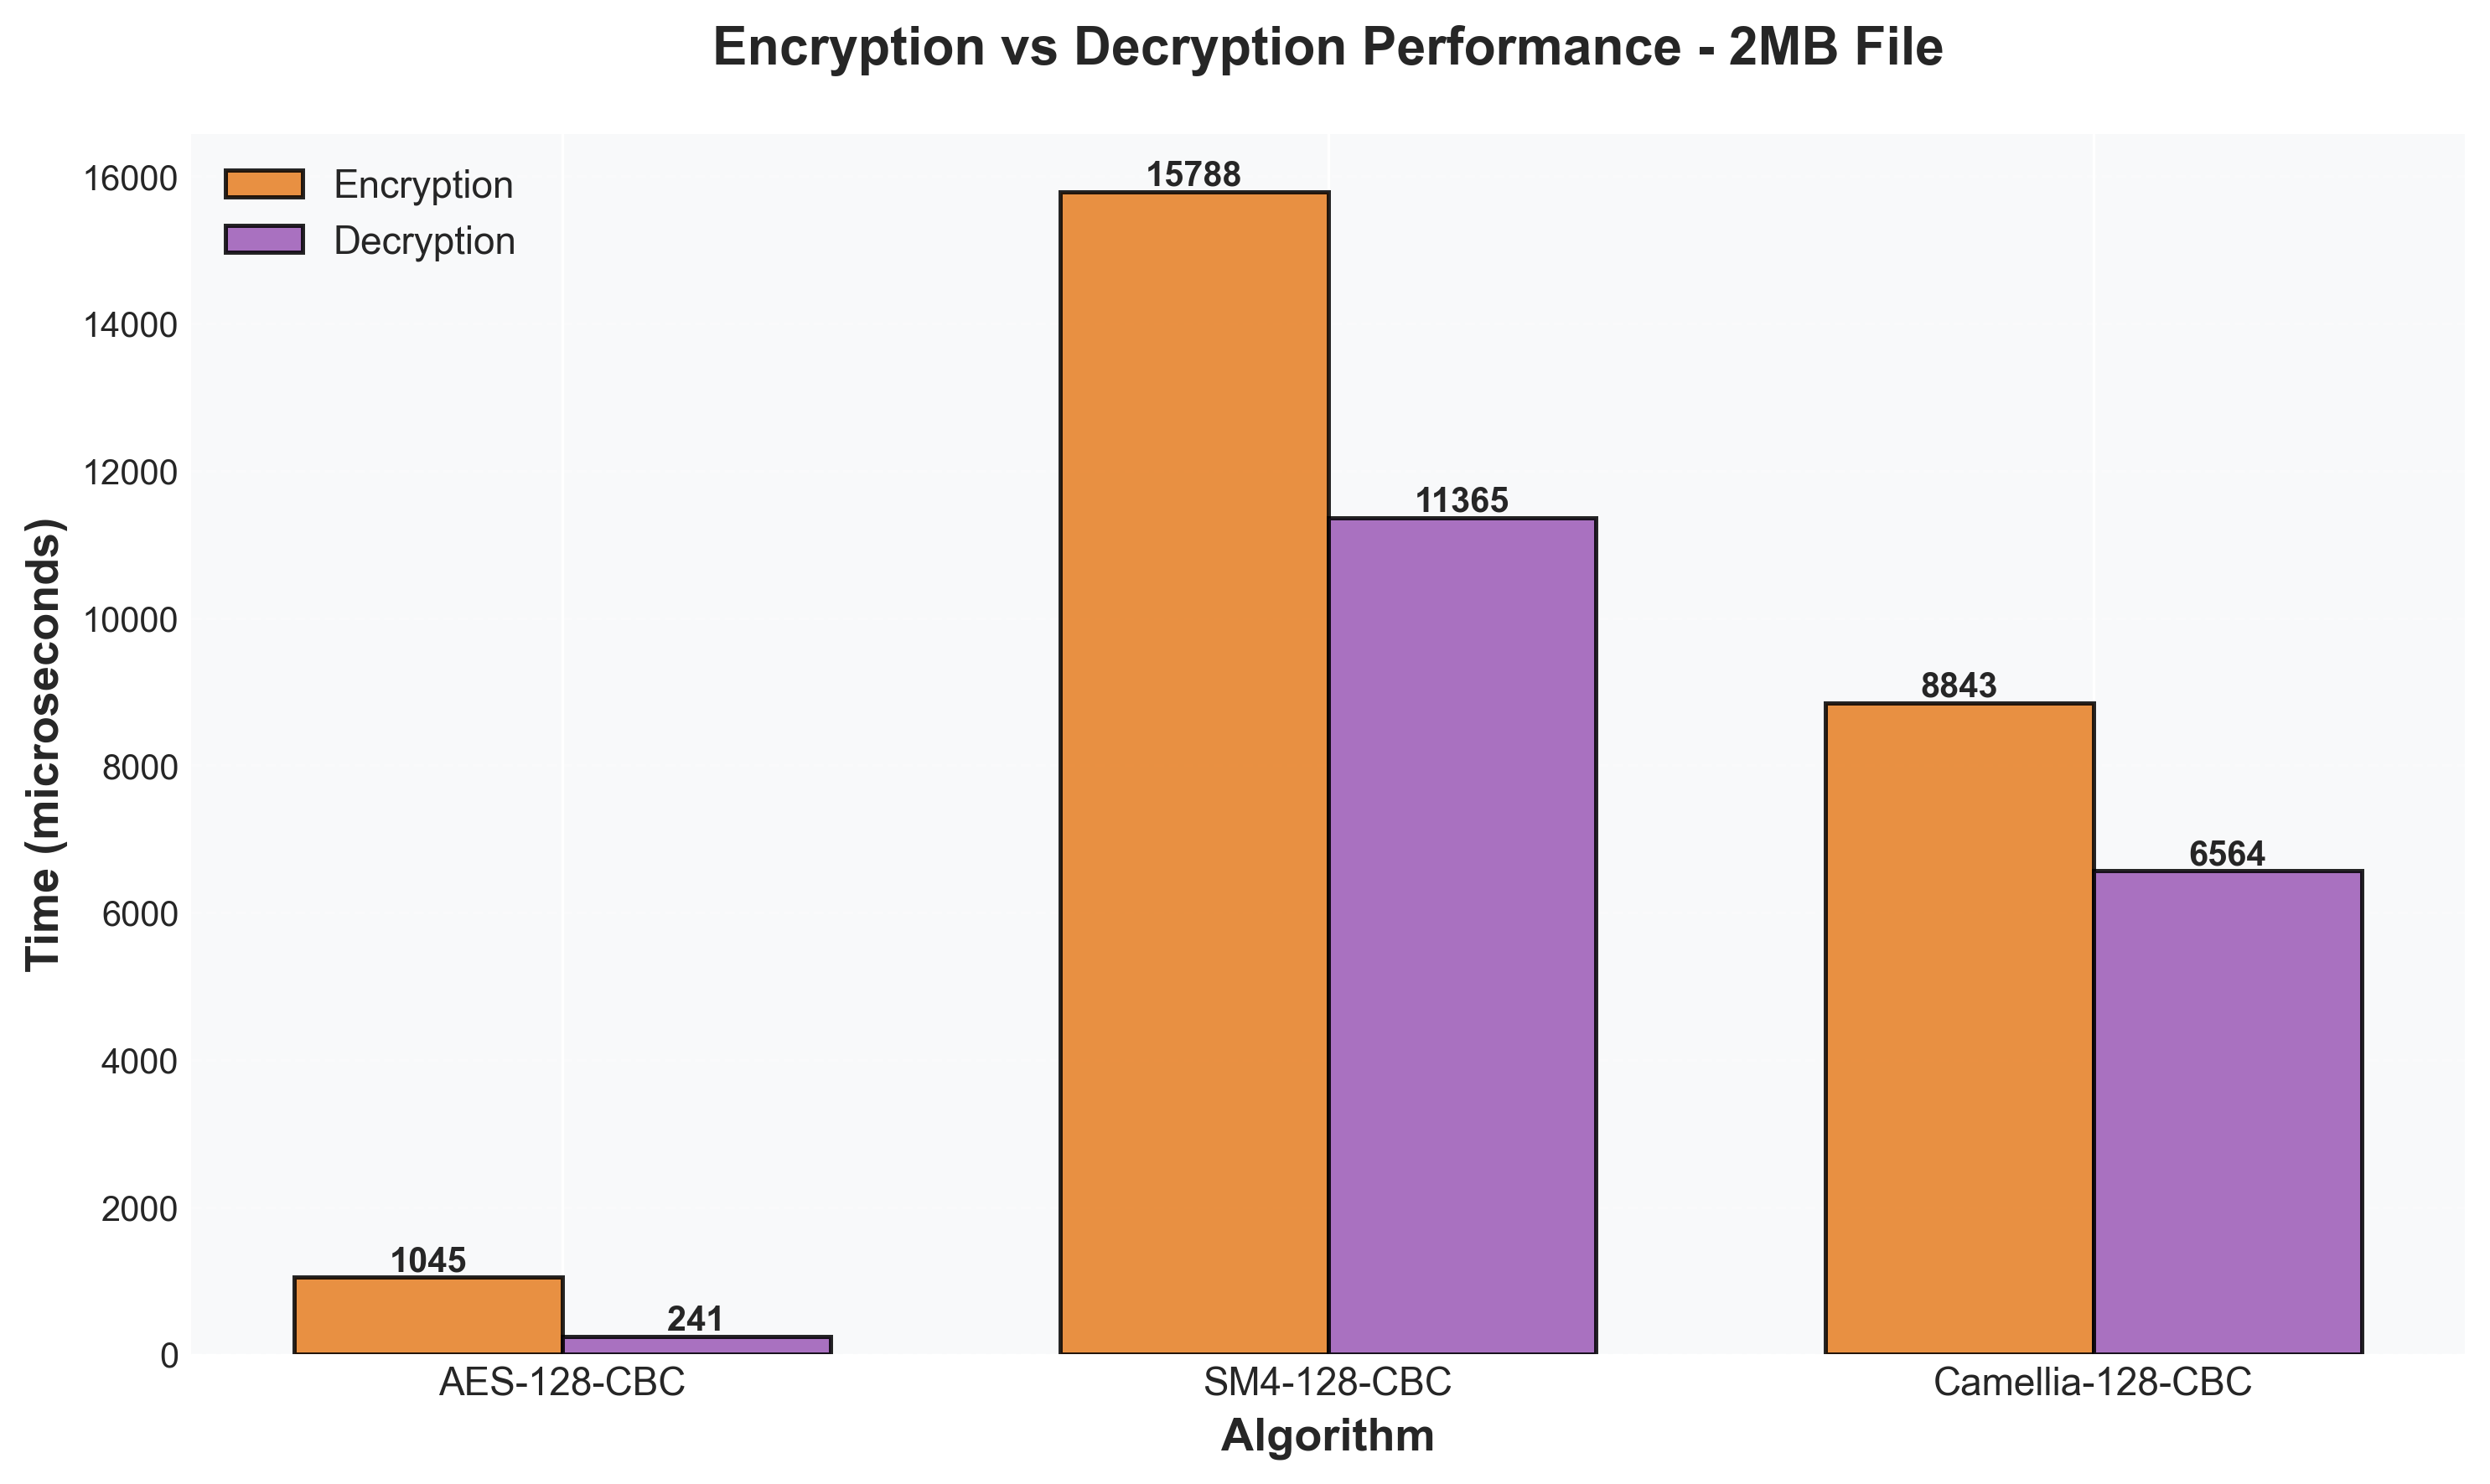
\includegraphics[width=0.85\textwidth]{performance_2MB.png}
\caption{Encryption and Decryption performance for 2MB file. The performance gap widens significantly, with AES demonstrating substantial speed advantages over SM4 and Camellia.}
\label{fig:perf_2mb}
\end{figure}

Key observations:
\begin{itemize}
    \item AES maintains its performance advantage with approximately 15× faster encryption and 47× faster decryption compared to SM4
    \item Camellia performs approximately 1.8× better than SM4 for large files
    \item All algorithms show asymmetric performance, with decryption generally faster than encryption
    \item AES's exceptional decryption speed (241 $\mu$s) suggests highly optimized parallel processing
    \item The performance gap between hardware-accelerated AES and software-only implementations (SM4, Camellia) becomes dramatic at scale
\end{itemize}

\subsubsection{Scalability Analysis}
Examining how performance scales with file size:
\begin{itemize}
    \item \textbf{AES}: Scales linearly and efficiently, approximately 1,913 MB/s encryption throughput for the 2MB file
    \item \textbf{SM4}: Shows linear scaling but at a lower throughput, approximately 126 MB/s encryption
    \item \textbf{Camellia}: Better than SM4 with approximately 226 MB/s encryption throughput
\end{itemize}

The consistent scaling behavior indicates that all algorithms are well-implemented, with the performance differences primarily stemming from algorithmic complexity and hardware optimization rather than implementation inefficiencies.

\subsection{Verification Results}
All encryption and decryption operations successfully passed verification tests. The \texttt{memcmp()} function confirmed that the decrypted data exactly matched the original plaintext for every algorithm and file size combination, demonstrating:
\begin{itemize}
    \item Correct implementation of encryption/decryption operations
    \item Proper handling of padding in CBC mode
    \item Data integrity throughout the encryption/decryption cycle
\end{itemize}

\newpage

\section{Conclusions}

\subsection{Final Remarks}
This homework demonstrated successfully the real performance factors of the three symmetric encryption algorithms we studied, highlighting that AES clearly dominates in terms of raw speed, while SM4 and Camellia remain viable options for specific use cases and platforms.

It is also very important to remember that the choice of encryption algorithm should consider not only performance (in terms of time) but also factors such as hardware support, standardization requirements and platform constraints.

All of the three algorithms analyzed provide strong cryptographic security and in many real-world scenarios, the performance differences observed here would be negligible compared to other system bottlenecks (disk I/O, network latency, etc.).

\end{document}